%%%%
%% Copyright 2022 Pierre S. Caboche
%% All rights reserved
%%%%

\part{Plots, Images, and Figures}


\section{Plots} \label{plots}

Plots are a very important component in \LaTeX, as they allow to draw all sorts of graphs. \\

Here is an example of chart that I used in another article:


\begin{figure}[h]
	\caption{An example of a bar chart}
	\centering
	\medskip

	\pgfplotsset{compat=newest}
	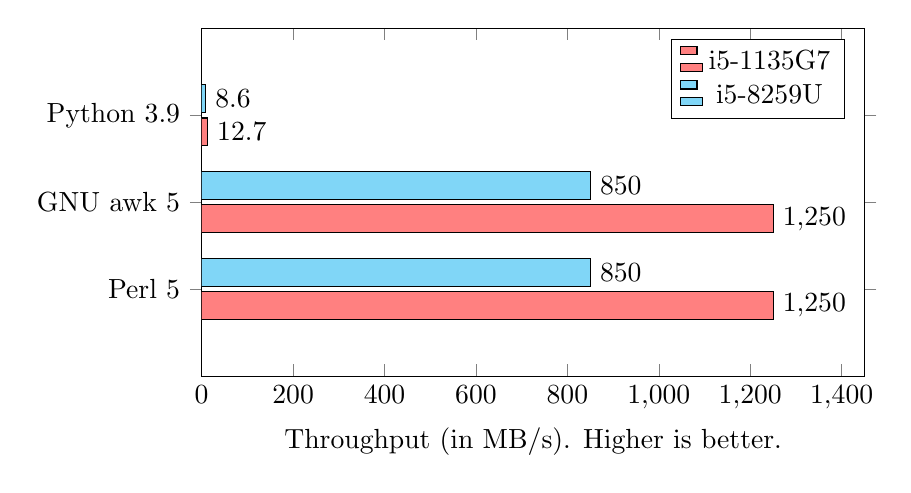
\begin{tikzpicture}
		\begin{axis}
			[ 
			xbar, 
			xmin=0, 
			width=10cm,
			height=6cm, 
			enlarge y limits=0.5, 
			xlabel={Throughput (in MB/s). Higher is better.},
			xmax=1450,
			%ylabel={Language},
			symbolic y coords={perl,gawk,python}, 
			yticklabels={Python 3.9,GNU awk 5,Perl 5},
			ytick=data,
			nodes near coords,
			nodes near coords align={horizontal}, 
			legend pos=north east
			]	
			\addplot[fill=red!50] coordinates {(12.7,python) (1250,gawk) (1250,perl)}; 
			\addplot[fill=cyan!50] coordinates {(8.6,python) (850,gawk) (850,perl)};
			\legend{i5-1135G7,i5-8259U};
		\end{axis} 
	\end{tikzpicture}
	\label{figure:throughput-comparison}
	
\end{figure}


\bigskip

To draw plots, you will need the \quotePkg{pgfplots} package:
\lstinputlisting[language=tex]{include/featured/pkg-pgfplots.tex}


We will not teach you how to draw plots, because the subject is extremely vast. \\



\section{Add an image}

We can add images to our \LaTeX\ files thanks to the \quoteCmd{includegraphics} command from the \quotePkg{graphics} package:
\lstinputlisting[language=tex]{include/featured/pkg-graphics.tex}


Example:
\begin{lstlisting}[language=tex]
\includegraphics{path/to/image-file}
\end{lstlisting}


\begin{figure}[h]
	\caption{Example: adding an image to a document}
	\includegraphics[keepaspectratio,width=\columnwidth]{files/texstudio.png}
\end{figure}


\bigskip

To learn more about \quoteCmd{includegraphics}: \\
\url{https://latexref.xyz/_005cincludegraphics.html}



\subsection{Resize an image to fit the page}

To resize an image to fit the page width, in \quoteCmd{includegraphics} we set the parameters \texttt{keepaspectratio} and \texttt{width}: \\

\begin{tabular}{p{3cm} p{9cm}}
	\texttt{keepaspectratio} & Will make the graphic as large as possible, without distortion, within the constraints of \texttt{width}, \texttt{height}. \texttt{totalheight}. \newline \\
	\texttt{width} & We set the \texttt{width} to either \quoteCmd{linewidth} or \quoteCmd{columnwidth}, and let \texttt{keepaspectratio} resize the image for us. \newline
	\newline
	\quoteCmd{linewidth}: the width of the current line, decreased for each nested list (but because we are not in a list, then it is equal to \quoteCmd{textwidth}, the horizontal width of the page body). \newline
	\newline
	\quoteCmd{columnwidth}: in a two-column document, the width of a column (in a two-column document, it is equal to \quoteCmd{textwidth}). \\
\end{tabular}

\bigskip

Example:
\begin{lstlisting}[language=tex]
\includegraphics[keepaspectratio,width=\columnwidth]{path/to/image-file}
\end{lstlisting}


\newpage


\section{Figures} \label{figures}

Figures are used for easy reference of plots, images, and other visual elements. Figures can be listed in a list of figures, usually at the end of a document. \\

We will study the code associated with figure \ref{figure:throughput-comparison}. \\


Here is the code in question:
\lstinputlisting[language=tex]{include/featured/example-plot-awk-speed.tex}



The content of a figure is contained in a \quoteEnv{figure} environment. The \texttt{[h]} indicates that we want to anchor the figure ``here" (at the location where it has been declared in the document). \\

Then we define the \quoteCmd{caption} of the figure (which will also appear in the list of figures, if one is defined in the document).

Then the command \quoteCmd{centering} indicates that the figure is to be centered in the page. \\

Then we insert the plot itself (which I am not going to describe, that would take too long).

Finally, after the plot, we insert a label. Notice that the ID for the figure starts with ``\texttt{figure:}". This is a convention which allows to easily identify the figures.


\section{List of figures}

We can easily add a list of figures (preferably at the end of the document) with the \quoteCmd{listoffigures} command:
\begin{lstlisting}[language=tex]
\listoffigures
\end{lstlisting}

